\section{mo\-Move\-Init$<$ M $>$ Class Template Reference}
\label{classmo_move_init}\index{moMoveInit@{moMoveInit}}
Move ({\bf mo\-Move}{\rm (p.\,\pageref{classmo_move})}) initializer.  


{\tt \#include $<$mo\-Move\-Init.h$>$}

Inheritance diagram for mo\-Move\-Init$<$ M $>$::\begin{figure}[H]
\begin{center}
\leavevmode
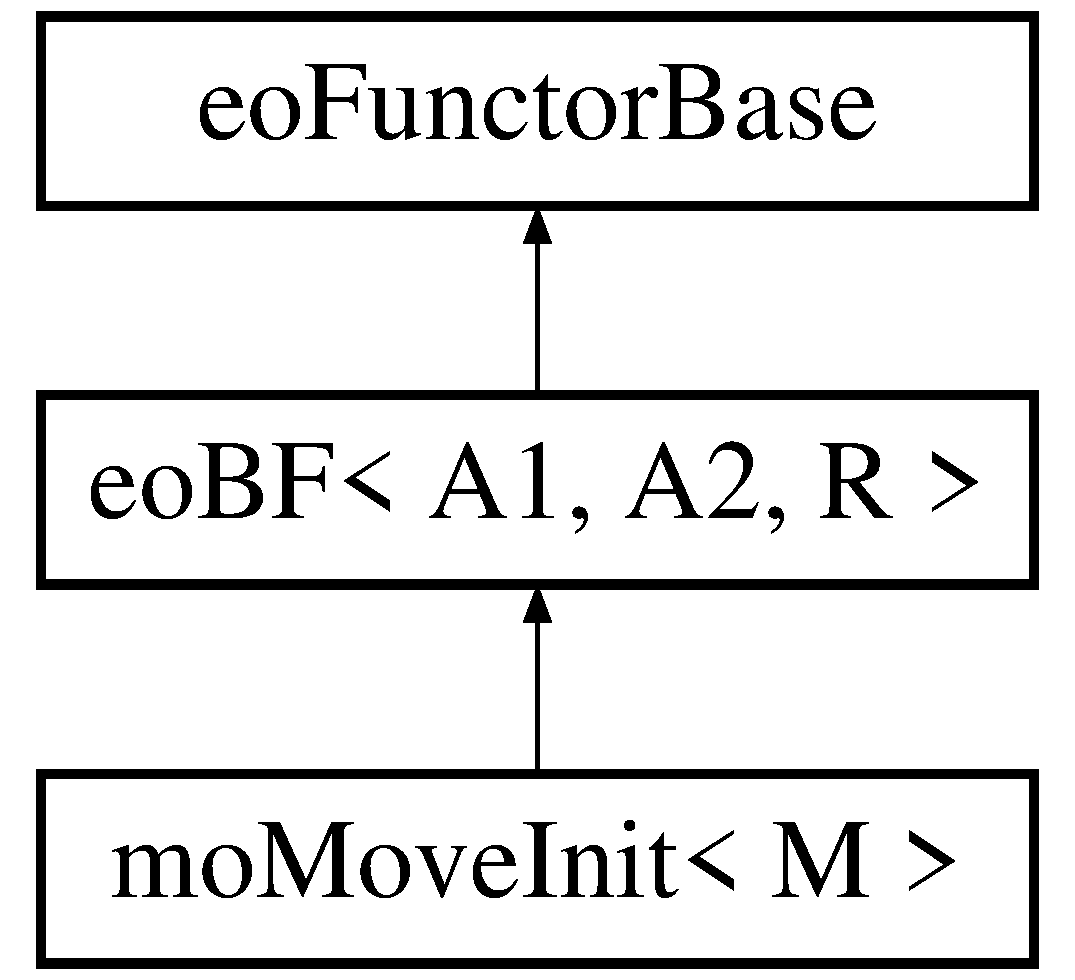
\includegraphics[height=3cm]{classmo_move_init}
\end{center}
\end{figure}


\subsection{Detailed Description}
\subsubsection*{template$<$class M$>$ class mo\-Move\-Init$<$ M $>$}

Move ({\bf mo\-Move}{\rm (p.\,\pageref{classmo_move})}) initializer. 

Class which allows to initiase a move. Only a description... An object that herits from this class needs to be designed to be used. 



Definition at line 47 of file mo\-Move\-Init.h.

The documentation for this class was generated from the following file:\begin{CompactItemize}
\item 
mo\-Move\-Init.h\end{CompactItemize}
